\documentclass[a4paper]{article}

%% Language and font encodings
\usepackage[english]{babel}
\usepackage[utf8x]{inputenc}
\usepackage[T1]{fontenc}

%% Sets page size and margins
\usepackage[a4paper,top=3cm,bottom=2cm,left=3cm,right=3cm,marginparwidth=1.75cm]{geometry}

%% Useful packages
\usepackage{amsmath}
\usepackage{graphicx}
\usepackage[colorinlistoftodos]{todonotes}
\usepackage[colorlinks=true, allcolors=blue]{hyperref}
\usepackage{algorithm}
\usepackage{algorithmic}
\usepackage{amssymb}
\usepackage{float}
\usepackage{caption}
\usepackage{subcaption}


\title{Chapter 1 - Introduction to Deep Learning}
\author{Viral Thakar}

\begin{document}
\maketitle
\section{Introduction}
\textbf{Intelligence}, one of the most important thing humans have acquired during the evolution. It is our ability to think abstractly, reason, establish correlation between experiences and convert them into knowledge, be creative, predict and most importantly to generate emotions. Human brain is always considered as one of the most complex and fascinating structures across all over the known universe because it is empowered by intelligence. If we try to understand more about the relation between brain and intelligence, we can realize that the brain is more like a tool which gathers informations from all of our senses and help our intelligence to enrich its capabilities. Human brain is simple just like any other organ but the intelligence is complex and we always try to understand the intelligence aspect of our brain. For example when we take decision to move our hand from hot plate, actually it is our intelligence which instruct our brain to move our hand and that is why it is often found that people with paralysis or in coma may not be able to control their body but shows all the signs of intelligence. In fact our intelligence is us, different from our body and unique compared to other human individuals.

\textbf{Artificial Intelligence} is a science and engineering to make intelligent machines as suggested by John McCarthy who has first coined this term in 1956. Modern era has evolved the definition of AI in context of computers by considering it as a domain to make intelligent programs for computers or computer operated systems. Just like human brain, computer also develops its intelligence from collected informations, we call it \textbf{Data}. As human brain collects data through basic senses i.e. sight, hearing, taste, touch, smell and proprioception, our intelligence is also different for each type of senses and our decisions or actions are outcomes of our collective intelligence. It is also important to observe that in general sight or vision is usually the most dominant sense we have and our collective intelligence is highly dependent on the visual information. We can understand the context of scene just by looking at it. We can perceive three dimensional world around us and differentiate shapes with ease. Researchers has found the concept of developing intelligence of computers using visual informations very interesting and this has lead us a domain of AI called \textbf{Computer Vision}. Formally computer vision is a sub-domain of AI where computers are being made intelligent enough to collect visual information from real world in form of images or videos and develop their high-level understanding about the world. 

\textbf{Learning} is a task of converting collected information or data into intelligence, knowledge or expertise. Researchers have found that it is easy to develop artificial intelligence where the relation between collected information and decision or action taken can be represented by some set of mathematical rules. The hard part is the decisions or actions we take intuitively. The bottleneck of the AI is to find mathematical representations of our intuitive decisions or actions withe respect to collected information like understanding speech, understanding objects with deformations. The goal of this book is to develop and understand Learning algorithms for such intuitive decisions taken based on visual informations. 

Let's understand different keywords like Deep Learning, Machine Learning, Knowledge base Learning, and Representation Learning which we frequently use in this particular domain and how they are related to AI. To understand this let's consider an example where we want to develop a program which can identify difference between Cats and Dogs. The very first step is the collection of information or data. To collect data, let's assume that we physically get thousand cats and dogs each, randomly from the market. Next We can start collecting information either in form of Textual Description or by taking images of each. As we want to get into computer vision we take images as data and which makes our problem an Image Classification problem. So at this point I have total two thousand images of cats and dogs. We need few samples to test our performance so we can divide our two thousand samples into 80\% (1600 images)for training and call them Training Set and 20\% (400 images)for testing and call them Testing Set. 

The first approach we can come up with is we take each image from our test set, and start matching it with every single image in training set. If we are able to find a matching image in training set, we assign a class label i.e. cat or dog, same as the matched image in the training set. This approach to AI is called \textbf{Knowledge Base Learning} where the training set act as knowledge or intelligence of our program. The problem with this approach is we need a huge training set to cover all the images in test set. Also there is a possibility of getting a species of cat or dog which is not part of our training set or we come across an image taken from different angle. 

To solve the problems associated with knowledge base learning, we can find significant pieces of information known as \textbf{features} e.g. ears, nose, face, paw etc which help us as humans to understand difference between cats and dogs and code functions to find these features from image. This set of features will be our intermediate training data. We create a program which takes this set of features as input and has ability to extract the hidden patterns from it to associate them with label. This approach to AI is called \textbf{Machine Learning} where the AI has capability to find hidden patterns from a given set of features representing the data. Despite of its success into certain domains like numerical data analysis, predicting type of cancer, predicting stock prices etc, the machine learning was not enough to develop an AI which can understand objects in image. The reason behind this limitation is our limitation to understand and find exact set of features which can collectively represent the given object. The manual process of finding the set of features is called \textbf{Feature Engineering}. In other words the machine learning systems depends heavily on the effectiveness of methods chosen during feature engineering.  

The difficulties faced by systems based on machine leaning suggest that AI system needs the ability to not only acquire knowledge by extracting hidden patterns from given data but also acquire set of features to represent the given data points. This ability to acquire set of features to represent the given data is called \textbf{Feature Learning} which replaces the manual feature engineering part. This approach to AI is called \textbf{Representation Learning} where we use machine learning to extract features as well as to establish mathematical relation between extracted features and output labels. With context to our experiment, when we decide to feed the training images as it is and let our program to figure out which is the best set of features to classify the images. For example coming up with some sort of generalized, high-level, abstract features like contours which represents shape of cats and dogs with every minute details. This complexity of representation learning has given rise to an approach to AI called \textbf{Deep Learning} where we decide to represent this high level, abstract representation into a collection of internally correlated simpler representation. It is similar to form a deep graph which represents the contextual correlation between simpler representations of the given image. For example a given image can be represented as a set of small parts, each part can be represented as a set of contours, each contour can be represented as a set of edges and so on. Refer Figure 1.1 for the illustration of Deep Image Classification Network VGG16 layer visualization.         

\begin{figure}[H]
\centering
\begin{minipage}{.5\textwidth}
  \centering
  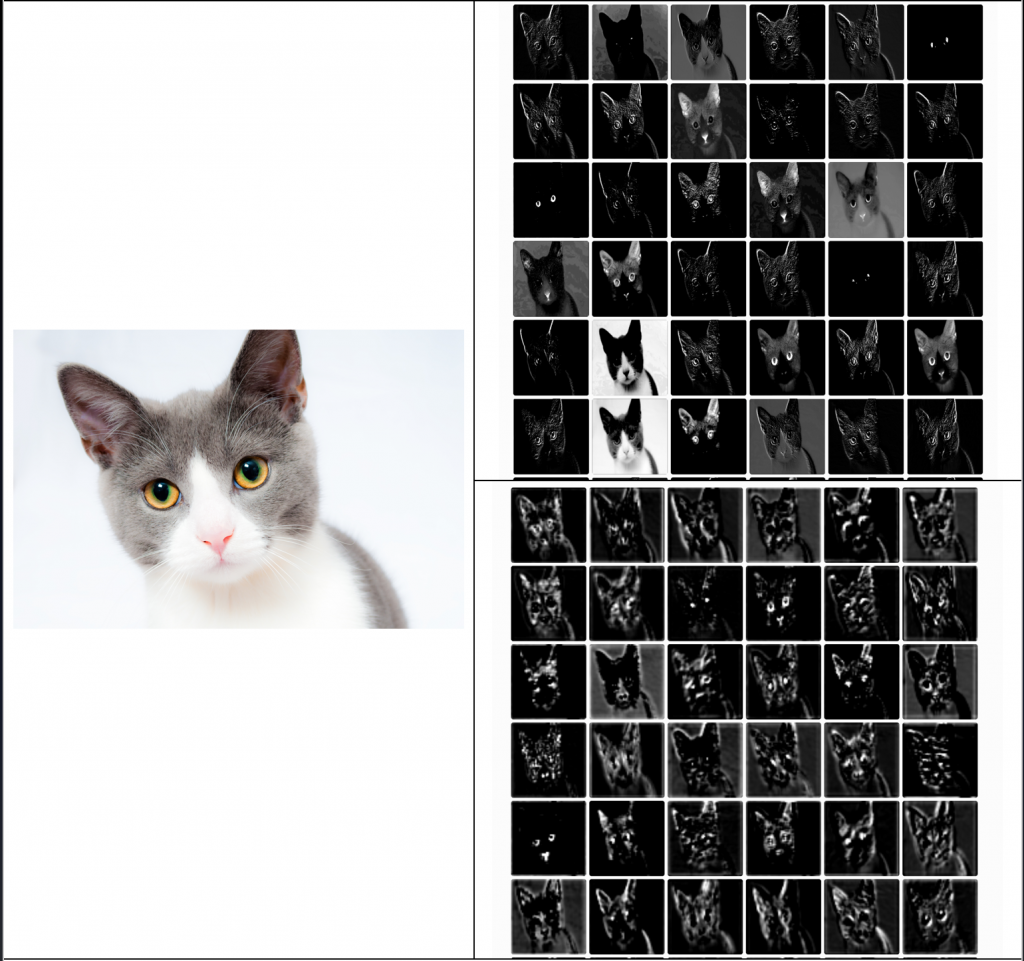
\includegraphics[width=0.4\linewidth]{images/cat.png}
\end{minipage}%

\begin{minipage}{.5\textwidth}
  \centering
  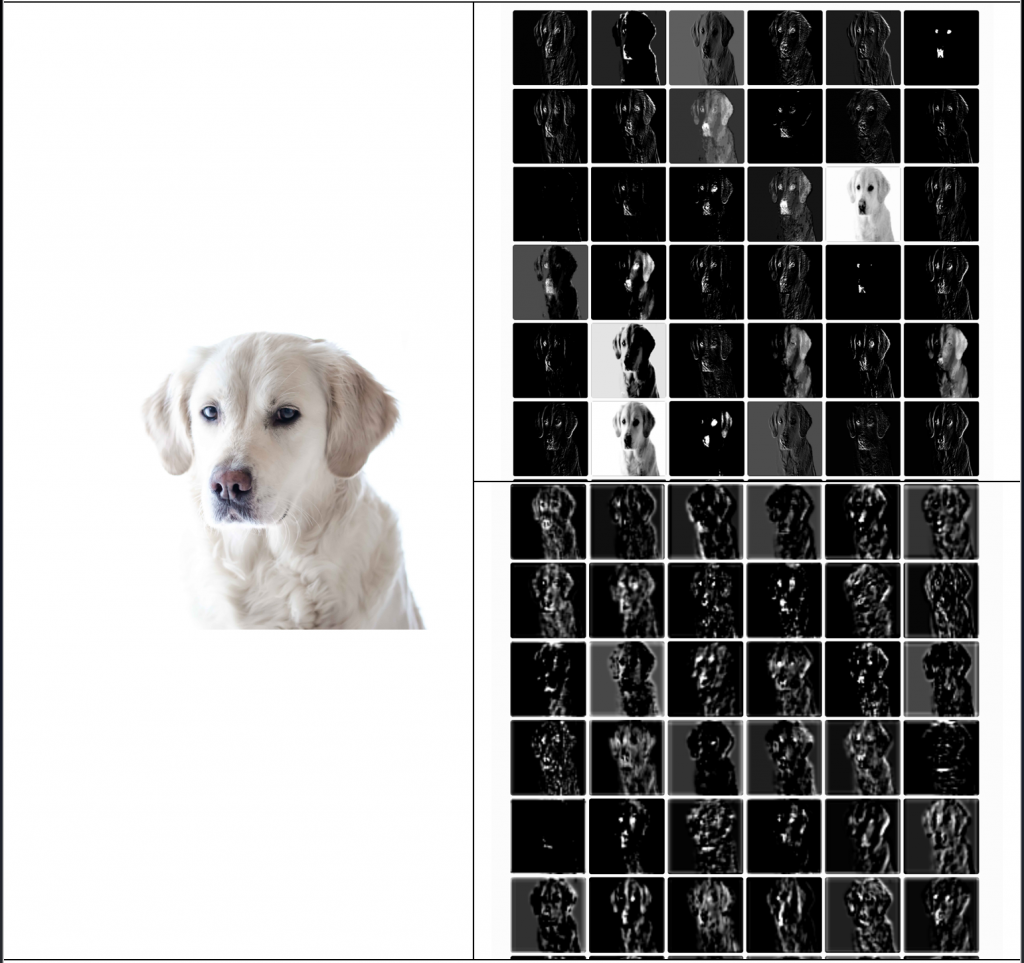
\includegraphics[width=.4\linewidth]{images/dog.png}
\end{minipage}

\caption{Illustration of VGG16 network for an image of cat and dog. It shows how Deep Learning divide the task into different representations. The representations in the top shows the lower level features like edges and bottom images shows higher level features like contours. 
}
\label{fig:1.1}
\end{figure}


\section{When and Why Do we Use Deep Learning}
Deep Learning is like a big hammer, which every nail doesn't require. Every deep learning based approach requires a decent amount of resources to implement in research and quite more resources to use it in production. That is why it is very important to understand what type of problems requires a deep learning based approach and when we can solve the given problem just by using simple machine learning tools. In general we can divide the problems based on two criteria : Their complexity to select features and their requirements for generalization or adaptivity. 

Let's consider a problem where a Birdwatcher wants to understand food behavior of five different bird species based on following set of information : (i) Length of beak (ii) Shape of beak (iii) Image of each birds (iv) Sound of each bird (v) Labels for food behavior category. The first step for us is to understand the given problem. We want to classify birds according to their food behavior. Through basic review about the domain we can easily find that there is a strong relation between type of beak (Length and Shape) and food behavior of a bird. There can be different approaches to solve this problem. 

\begin{enumerate}
\item Using Machine Learning : We take Length of beak and Shape of beak as features and design a classifier which can classify the birds into different classes according to their food behavior. 
\item Using Deep Learning : We take the images of birds and classify them into different classes according to their food behavior.   
\end{enumerate}

We can easily see that in this particular problem Machine Learning based approach is much more easy and should be more accurate because the features we are providing are the exact set of features to classify birds according to their food behavior. 

Next our Birdwatcher ask us to group birds based on their similarity in voice and appearance. While approaching this problem we realize that sound of birds changes according to time, weather and their mood. Same way it is very hard to characterize unique features to describe and differentiate appearance. For this type of problem Deep Learning is a more suitable tool. 

To summarize, Deep Learning is great for 
\begin{itemize}
\item Problems which require large number of features to solve, and it is hard to describe each feature. e.g. recognizing voice, recognizing faces
\item Problems which requires inter-correlated features to build higher level understanding e.g. semantic analysis of sentences, object tracking and segmentation, document summarization
\item Problems which requires high adaptiveness
\end{itemize}

\section{Types of Learning}
As described earlier Learning is a process of converting experience into knowledge, expertise or intelligence. It is a very wide domain but with reference to AI we can classify them into four broad categories. 

\subsection{Supervised, Unsupervised, Semi-Supervised and Reinforcement Learning}
This four categories are based upon one criteria : Relation between Learner and Environment. In other words how much learner is familiar with the environment with the help of human supervision. Consider set of problems provided by the Birdwatcher. In first problem to classify birds based on food behavior we considered a system where our learner has access to training data with labels. In this condition the goal of our learner is to come up with a set of rules which Birdwatcher can use to classify any new test sample. On other side in second problem we have to group similar birds based on their sound and appearance. There was no direct label available, literally there was no distinction between training and testing data. 

Precisely \textbf{Supervised Learning} is a type of learning where environment provides enough supervision on the performance of learner as during learning part it knows the missing piece of information which is label. In contrast \textbf{Unsupervised Learning} is a type of learning where there is no supervision available from environment or in other words there are no label available for training dataset. When we combine this two approaches where we provide a very little supervision and most of the learning occurs unsupervised, it is called \textbf{Semi-Supervised Learning}. For example for the second problem by Birdwatcher, we can group the birds using unsupervised learning and then assign labels to each group so that in future we can treat the problem as supervised learning problem. Similar approach is used in Apple or Google Photos while it recognizes person in the images.

\textbf{Reinforcement Learning} is totally different approach to learning. It is more similar to humans where learner or known as agent observes the environment, understand its state, takes particular action and based on the reward it receives in return it learns its performance in that particular combination of environment, state and action. By repeating this steps for set of possible different states and associated actions learner learns a best suitable strategy aka policy to get the most reward over time. \textbf{Policy} is an optimal strategy to achieve optimal reward for the given environment with available set of states and actions. It defines which action the agent is supposed to take for a particular state to maximize the reward. 

\subsection{Batch and Online Learning}
This two categories are based upon the learning capability of learner : whether it is able to change rules it has learned on-line, continuously, throughout the learning process or it needs a large amount of data access before deciding a set of rules. For example while learning about stock prices our learner needs a capability to adapt its rules daily based on the past as well as today's experience. It can make its set of rules better over the period of time by having more experience but ability to update rules based upon the current data makes the learner an on-line learner. On other side while classifying birds we don't explicitly need to update our learning on the fly and we can use a batch learner.

\subsection{Active and Passive Learning}
This two categories are based on the role learner plays during the learning process. Active learner is a type of learner which interacts with the environment by posing queries or performing different experiments to improve its understanding while the passive learner waits to receive information and only observe the provided information. For example for the second problem suggested by Birdwatcher if we design a learner which at some interval of time comes up with pairs of images and ask the Birdwatcher to classify them either matching by appearance or not matching then the behavior of learner is Active.  

\subsection{Knowledge Based and Model Based Learning}
This two categories are based on whether learner remembers all the training data by heart or create a model using the training examples to predict future instances. If the learner remembers all the training examples and uses similarity measure to find output for new test instances then the learning approach is known as Knowledge based learning. In contrast a learner which creates a model from the training samples and use that model to predict output for the new test instance is called Model based learning. 

Apart from this four categories, there is also a whole new class of learning algorithms exists where the input to learner is generated from Adversarial environment which we will discuss more in chapter 9 of this book. This book focuses more on the algorithms based on Supervised Learning, Batch Learning and Passive Learning. It also covers other types of learners for very specific algorithms only.  


\section{Recent Trends in Deep Learning}
Deep Learning is becoming one of the top most used buzz word because of its unmatchable performance in tasks like image recognition, speech recognition, object detection and tracking, natural language processing etc. Figure shows the trend of Deep Learning, Machine Learning and Artificial Intelligence search terms from 2004 to 2017, world wide by Google trends. 

\begin{figure}[H]
\centering
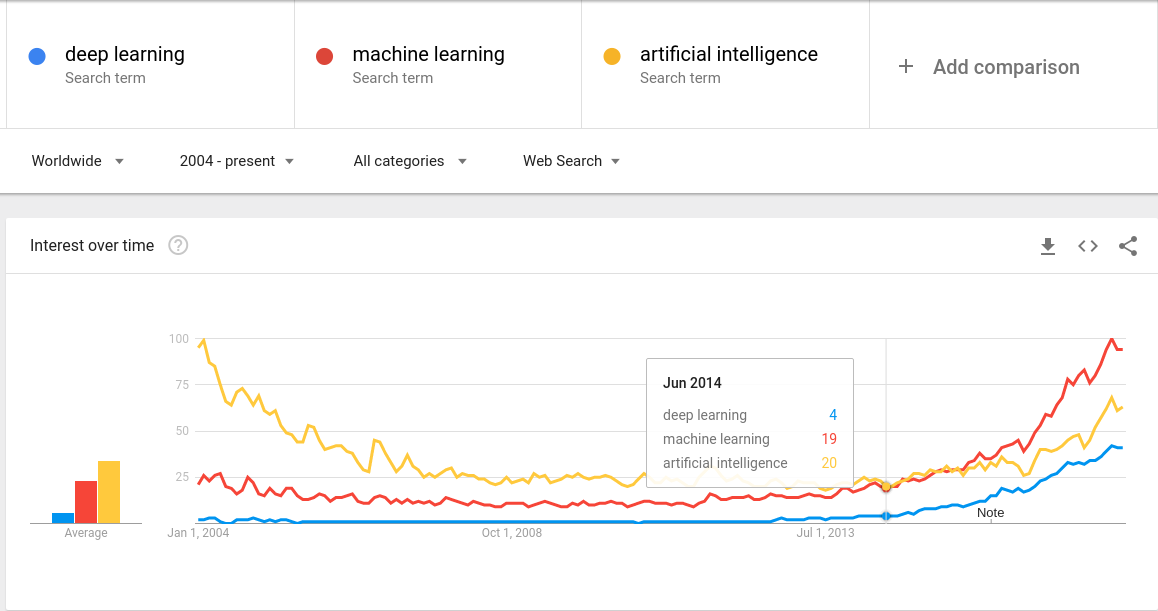
\includegraphics[width=\linewidth]{images/Trend_ml_ai_dl.png}
\caption{Interest over Time curve generated using Google Trends for Deep Learning, Artificial Intelligence and Machine Learning search terms since 2004 to 2017.  
}
\label{fig:1.2}
\end{figure}

It clearly shows some real good insights about these terms and how they are evolving in the time-line. Back in time Artificial Intelligence is the term which was most popular and represents all type of algorithms which were designed to make machines intelligent. But as you can see almost around Jun 2014 the Machine Learning has started dominating the field of Artificial Intelligence by making computer programs smarter and independent from any human supervision. Deep learning is a domain which has started evolving somewhere around 2012 and then onwards it is continuously growing its popularity in almost all the categories. This also provides us an insight that in recent years growth of AI has major contributions from growth in machine learning and deep learning. In fact these three domains are not competitive among each other rather they are collaborative, machine learning and deep learning co-existing under the umbrella called AI. Deep learning is nothing but one of the possible ways to make machine learning possible.

Deep Learning represents large, deep, neural network where deep represents multiple layers of neurons. We will discuss more about Artificial Neural Networks and Deep Neural Networks in chapter 3 but right now for simple understanding we can say that the idea of artificial neural networks is highly inspired by the model of how neurons function in human brain. To model the behavior of 'connectionism' displayed by neurons in human brain, in 1943 Warren McCulloch and  Walter Pitts came up with a mathematical model under the title "A logical calculus of the ideas immanent in nervous activity". In 1957 Frank Rosenblatt has set the foundation of modern day deep neural networks by making the McCulloch-Pitts Neuron a reality in form of "Mark - 1 Perceptron". The key contribution of Mark 1 Perceptron was its ability to update its weights by minimizing the difference between desired output and actual output. In 1960 Bernard Widrow and Marcian Hoff came up with a different approach to Perceptron by returning weighted input as output. In 1969, book called "Perceptrons" by Marvin Minsky and Seymour Papert has challenged Rosenblatt's single perceptron by showing its limitation to solve very famous XOR function or in general non-linear functions. Almost a decade after this publication is know as THE AI WINTER when there was almost no funding to push the research in Neural Networks.

In early 80's the second wave of neural networks began when Jon Hopfield presented his paper on Hopefield Net which has laid foundation for modern day Recurrent Neural Networks. The major breakthrough was Geoff Hinton, David Rumelhart and Ronald William's paper entitled as "Learning representations by back propagating errors" where they suggested the concept of \textbf{Back-propagation}. The main contribution of back-propagation was easy and efficient training of neural networks with many hidden layers which has helped to solve the problem associated with Mark 1 Perceptron. Back-propagation involves two main steps : Calculation of derivatives of network's loss function and back propagating the errors to update the weights and biases in each layer of network. In the same year Geoff Hinton, James McClelland and David Rumelhart suggested the concept of \textbf{distributed representation} where the concept is to represent each input into a set of features and those member features can be used to represent other inputs also. The major accomplishment of this phase in Deep Neural Networks was the first use of Convoluational Neural Networks with back-propagation to recognize hand written digits by team at AT\&T Bell Labs headed by Yann LeCun. This second wave of Deep Neural Networks lasted till mid 90's. There were many noticeable contributions during 90's like Hochreiter and Schmidhuber introduced Long Short term Memory network (LSTM Network) in 1997, and "Gradient Based Learning Applied to Document Recognition" by Yann LuCan, Leon Bottou, Patrick Haffner and Yoshua Bengio. Also in 1995, Corina Cortes and Vladimir Vapnik introduces Support Vector Machines which were real competitors of Neural Networks and even today researcher are using them for many tasks. 

Though deep  neural networks were showing potential capabilities in various domain, because of their huge computational and data requirements they were considered to be very difficult to train and use into production. The third wave of modern day deep neural networks began in 2006 when Geoffrey Hinton published ideas of Deep Belief Nets and Unsupervised pretraining or greedy layer-wise pretraining. The idea is to train a simple 2 layer unsupervised model like a restricted boltzman machine, freeze all the parameters, put a new layer on the top of them and train the parameters for the new layer only. This was the beginning of modern day Deep Neural Networks branded as Deep Learning. 

In 2009 team lead by Fei-Fei Li has launched ImageNet, which is even today one of the largest and free labeled dataset with 14,197,122 images distributed over large variants of labels. The dataset is associated with Large Scale Visual Recognition challenge where participants share their models trained and tested on ImageNet dataset. In first two years of LSVRC the top models had error rates of 28\% and 26\%. In 2012 Alex Krizhevsky, Ilya Sutskever and Geoffrey Hinton proposed a CNN model which had the error rate of 17\%. The key contribution of this submission is proposal of various key components like ReLU, Overlapping Pooling, Training on Multiple GPUs, Local Response Normalization, and Dropout which has improved performance of deep neural networks by a great margin. In true sense AlexNet has kick-started the Deep Learning revolution which we are experiencing right now. In 2013 the team of DeepMind Technologies has published a paper entitled as "Playing Atari with Deep Reinforcement Learning" which has used a variant of Q-learning called Deep-Q-Learning which is a major breakthrough in the domain of reinforcement learning. In the same year OverFeat - an object detection framework based on DNN and DLT Tracker - The first visual tracker based on DNN was published and started the expansion of deep learning in other domain of computer vision like object detection and tracking. 

Since 2014, the research in the domain has become so much intense that almost every approach or algorithm proposed was new and can be considered as breakthrough. In domain of Image Recognition VGGNet(2014), GoogleNet(2015), ResNet(2015) has out performed all the results for ILSVRC. These networks are deeper and computationally complex but advances in GPUs has supported their use even in production also. Image Captioning has started getting noticed in 2010 but got its major breakthrough in 2014 by papers like "Deep visual-semantic alignments for generating image descriptions" and "From captions to visual concepts and back". There was lot of contribution to Image Captioning in the year of 2014. Algorithms like RCNN(2014), Fast RCNN(2015), Faster RCNN(2015) has started to establish their dominance in object detection. Though these algorithms are very accurate for object detection even today, their speed is quite law compared to real-time object detection requirement. This limitation has given rise to YOLO(2015) and SSD(2015) object detection algorithms which are accurate and real-time. 2015 was more likely a year of Object Detectors. In 2016 Microsoft has achieved state of art performance in speech recognition. There was also a ground breaking concept of Synthetic Gradients has been introduced in same year under the paper entitled as "Decoupled Neural Interfaces using Synthetic Gradients". The major breakthrough of 2016 was popularity of AlphaGo - Mastering the game of GO with deep neural networks and tree search. There was also various major research contributions happed in the same year in the domain of reinforcement learning. In my opinion 2016 was more likely the year of Reinforcement Learning. In parallel there is a separate branch of unsupervised learning has evolved known as Deep Generative Models which includes Ian Goodfellow's Generative Adversarial Networks (GANs)(2014), DCGAN(2015), DRAW - A recurrent neural network for image generation (2015) and PixelCNN(2016). At the time of writing this book the most recent and major breakthrough of 2017 is the Capsule Nets by Sara Sabour, Nicholas Frosst, and Geoffrey Hilton.


\section{General Mathematical Model of Learning}
In this section we try to understand mathematically how we can define the learning problem or in general learner's behavior. By behavior we try to figure out how an input and output of a learner looks like and  how it establish relation between input and output. To understand and begin we will consider a supervised learning problem where we want set of rules to classify a given input. 

\subsection{Input to Learner}
Based on simple understanding we can establish that a Learner is supposed to have access to following information about the learning problem. 

\begin{itemize}
\item A set of all possible objects we wish to input to learner - Domain set
\item A set of possible labels or outputs - Label set
\item A training set which is made of few samples taken from Domain set along with appropriate label taken from Label set - Training set
\end{itemize}

\paragraph{Domain Set :}  It is an arbitrary set, $X$, which represents a set of objects we may wish to classify by assigning a proper label. For example a set of all possible birds with their beak length and shape represents the Domain set for the first Birdwatcher problem we have discussed in previous section. The member of domain set is called domain points or instances and they usually represents the feature vector. 

\paragraph{Label Set :}  It is a set of all possible Labels for a particular learning problem and represented as $Y$. Let's assume that for the first Birdwatcher problem we would like to classify birds into five categories : Meet Eater, Seed Eater, Food-Nut Eater, Fish Eater and Nectar Feeder. Let's represent each with an integer value ranging from 1 to 5. Then in this particular case our Label set $Y = \{1, 2, 3, 4, 5\}$.

\paragraph{Training Set :} It is set of fixed length sequence of pairs in $X \times  Y$ represented as $S = \{(x_1, y_1), .... , (x_m, y_m)\}$. It represents a finite length sequence of labeled domain points or instances. Learner has access to this input. It is also commonly known as Training Data or Training Examples. 

\subsection{Output of Learner}
The learner provides a set of rules which can be used to represent the relation between the input feature vector which is again from domain set and output label which is member of label set. This set of rules is called a hypothesis function or predictor and represented as $h : X \rightarrow Y $. 

\subsection{Routine of Learner}
The routine or learning process of a learner, first and foremost requires an exact parameter to measure the performance of learner or in other words to measure the error of learner. The overall goal of the whole learning process is to minimise this error. The error of a learner can be defined as the probability that the learner doesn't generate a correct label for a randomly generated data point or feature vector. 

Mathematically, the error of $h$ is defined as the probability to take a random feature vector x according to some probability distribution $D$, such that $f(x)$ is not equals to $h(x)$. 

$$ L_{D,f}(h) = P_{(x \sim D)}(h(x) \neq f(x) )  $$
where $D$ is a function which represents the distribution of possible feature vectors and $f$ is a true labeling function. 

The ultimate goal of Learning task is to come up with a hypothesis or predictor function $h$ which is as much close as possible to $f$ or in other words produces minimum $L$ for given $D$ and $f$. 


\section{Summary}
\begin{itemize}
\item Intelligence is our ability to think abstractly, reason, establish correlation between experiences and convert them into knowledge, be creative, predict and most importantly to generate emotions.
\item Artificial Intelligence is a science and engineering to make intelligent machines.
\item Learning is a task of converting collected information or data into intelligence, knowledge or expertise.
\item Machine Learning is an approach to AI where the AI has capability to find hidden patterns from a given set of features, representing the data.
\item The manual process of finding the set of features is called Feature Engineering.
\item This complexity of representation learning has given rise to an approach to AI called Deep Learning where we decide to represent this high level, abstract representation into a collection of internally correlated simpler representation.
\item Supervised Learning is a type of learning where environment provides enough supervision on the performance of learner as during learning part it knows the missing piece of information which is label.
\item Unsupervised Learning is a type of learning where there is no supervision available from environment or in other words there are no label available for training dataset.
\item The ultimate goal of Learning task is to come up with a hypothesis or predictor function  which is as much close as possible to  or in other words produces minimum  for given  and . 
\end{itemize}



\section{Further Reading}
\begin{itemize}
\item LeCun, Y., Bengio, Y. and Hinton, G., 2015. Deep learning. Nature, 521(7553), pp.436-444. [PDF]
\item A Gentle Start, Shalev-Shwartz, S. and Ben-David, S., 2014. Understanding Machine Learning: From Theory to Algorithms. Cambridge University Press, pp. 33-41.
\end{itemize}















\end{document}